\documentclass[12pt,letterpaper]{article}
\usepackage[utf8]{inputenc}
\usepackage[spanish]{babel}
\usepackage{graphicx}
\usepackage[left=2cm,right=2cm,top=2cm,bottom=2cm]{geometry}
\usepackage{graphicx} % figuras
% \usepackage{subfigure} % subfiguras
\usepackage{float} % para usar [H]
\usepackage{amsmath}
%\usepackage{txfonts}
\usepackage{stackrel} 
\usepackage{multirow}
\usepackage{enumerate} % enumerados
\renewcommand{\labelitemi}{$-$}
\renewcommand{\labelitemii}{$\cdot$}
% \author{}
% \title{Caratula}
\begin{document}

% Fancy Header and Footer
% \usepackage{fancyhdr}
% \pagestyle{fancy}
% \cfoot{}
% \rfoot{\thepage}
%

% \usepackage[hidelinks]{hyperref} % CREA HYPERVINCULOS EN INDICE

% \author{}
\title{Caratula}

\begin{titlepage}
\begin{center}
\large{UNERSIDAD PRIVADA DE TACNA}\\
\vspace*{-0.025in}
\begin{figure}[htb]
\begin{center}

\includegraphics[width=8cm]{./Imagenes/logo}
\end{center}
\end{figure}
\vspace*{0.15in}
INGENIERIA DE SISTEMAS  \\

\vspace*{0.5in}
\begin{large}
TITULO:\\
\end{large}

\vspace*{0.1in}
\begin{Large}
\textbf{ Guia de Instalacion y Configuracion de Base de Datos} \\
\end{Large}

\vspace*{0.3in}
\begin{Large}
\textbf{CURSO:} \\
\end{Large}

\vspace*{0.1in}
\begin{large}
BASE DE DATOS II\\
\end{large}

\vspace*{0.3in}
\begin{Large}
\textbf{DOCENTE(ING):} \\
\end{Large}

\vspace*{0.1in}
\begin{large}
 Patrick Cuadros Quiroga\\
\end{large}

\vspace*{0.2in}
\vspace*{0.1in}
\begin{large}
Integrante: \\
\begin{flushleft}
Mamani Limache, Jhony 		\hfill	(2013046566) \\
Condori Tito, Hernan  		\hfill	(2009034553)\\
Moreno Caceres, Renzo Alex 	\hfill	(2013047246) \\
Ordoñez Quilli, Ronald 		\hfill	(2015052821)\\
apellido y nombre			\hfill	(codigo)\\
apellido y nombre			\hfill	(codigo) 
\end{flushleft}
\end{large}
\end{center}

\end{titlepage}


\tableofcontents % INDICE
\thispagestyle{empty} % INDICE SIN NUMERO
\newpage
\setcounter{page}{1} % REINICIAR CONTADOR DE PAGINAS DESPUES DEL INDICE


\section{Parte 01 - Definiciones} 

\begin{enumerate}[1.]
	\item Objetivos
	\\\\- Brindar al estudiante los conocimientos necesarios para realizar la Instalación de un servidor de Base de Datos Oracle sobre un sistema operativo Linux.	
	\\- Otorgar al estudiante los conocimientos necesarios para realizar la instalación de este servidor dentro de un ambiente virtualizado.\\
	\item Requerimientos
	\\-Conocimientos
	\subitem Para el desarrollo de esta práctica se requerirá de los siguientes conocimientos básicos:

	\item Consideraciones Iniciales.
	\subitem Tener conocimientos b\'asicos como usuario de Windows Server 2012 R2

	
	

\end{enumerate} 

\section{Parte 02 – Instalacion de VMWare} 

\begin{enumerate}[1.]
	\item Paso 01 : ejecutar el instalador de VMware y seleccionar en todas las ventanas el boton next
	
	\begin{center}
	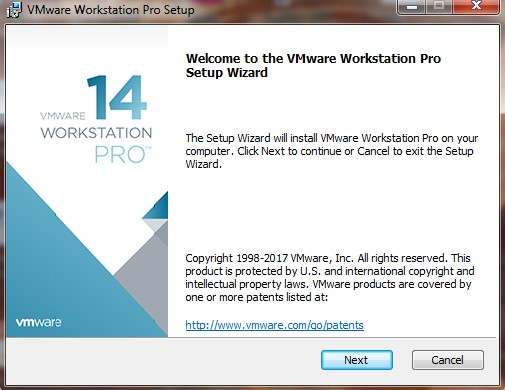
\includegraphics[width=15cm]{./Imagenes/WM01} 
	\end{center}

	\item Paso 02 :

	\begin{center}
	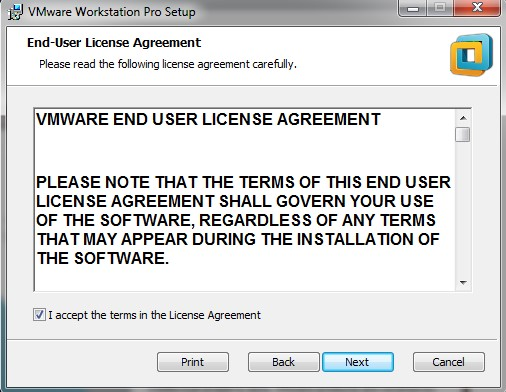
\includegraphics[width=15cm]{./Imagenes/WM02} 
	\end{center}

	\item Paso 03 :

	\begin{center}
	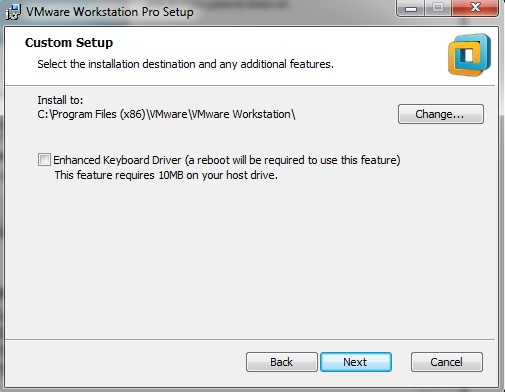
\includegraphics[width=15cm]{./Imagenes/WM03} 
	\end{center}

	\item Paso 04 :

	\begin{center}
	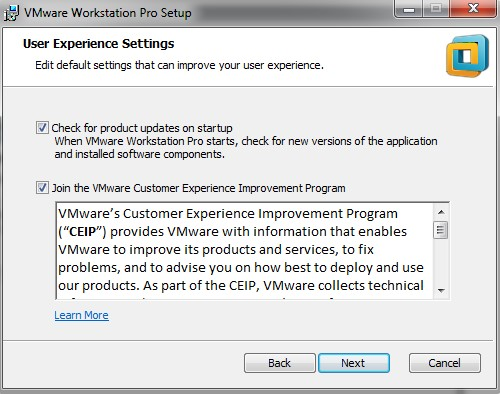
\includegraphics[width=15cm]{./Imagenes/WM04} 
	\end{center}

	\item Paso 05 : ahora ya instalamos el programa

	\begin{center}
	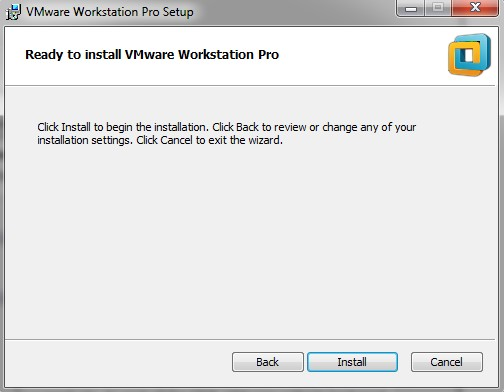
\includegraphics[width=15cm]{./Imagenes/WM05} 
	\end{center}

	\item Paso 06 :

	\begin{center}
	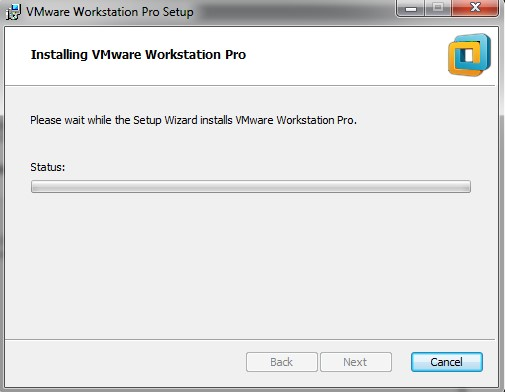
\includegraphics[width=15cm]{./Imagenes/WM06} 
	\end{center}

	\item Paso 07 :

	\begin{center}
	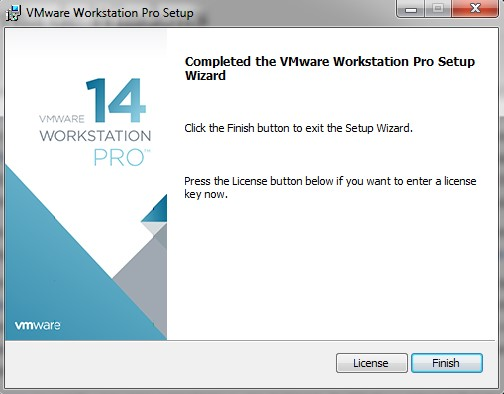
\includegraphics[width=15cm]{./Imagenes/WM07} 
	\end{center}

	\item Paso 08 : Ingresamos la clave del producto

	\begin{center}
	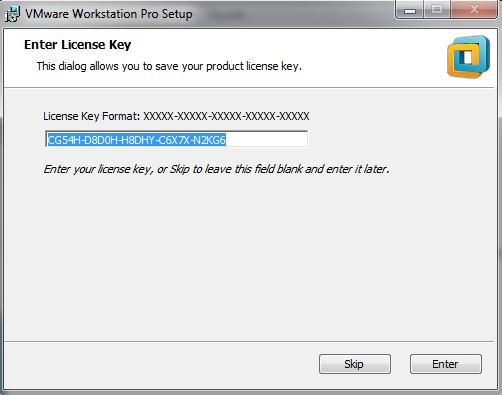
\includegraphics[width=15cm]{./Imagenes/WM08} 
	\end{center}

	\item Paso 09 :

	\begin{center}
	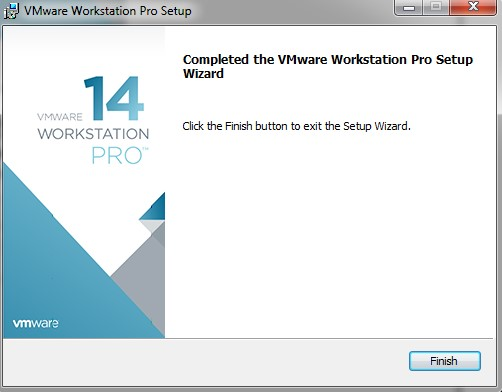
\includegraphics[width=15cm]{./Imagenes/WM09} 
	\end{center}

	\item Paso 10 : Listo

	\begin{center}
	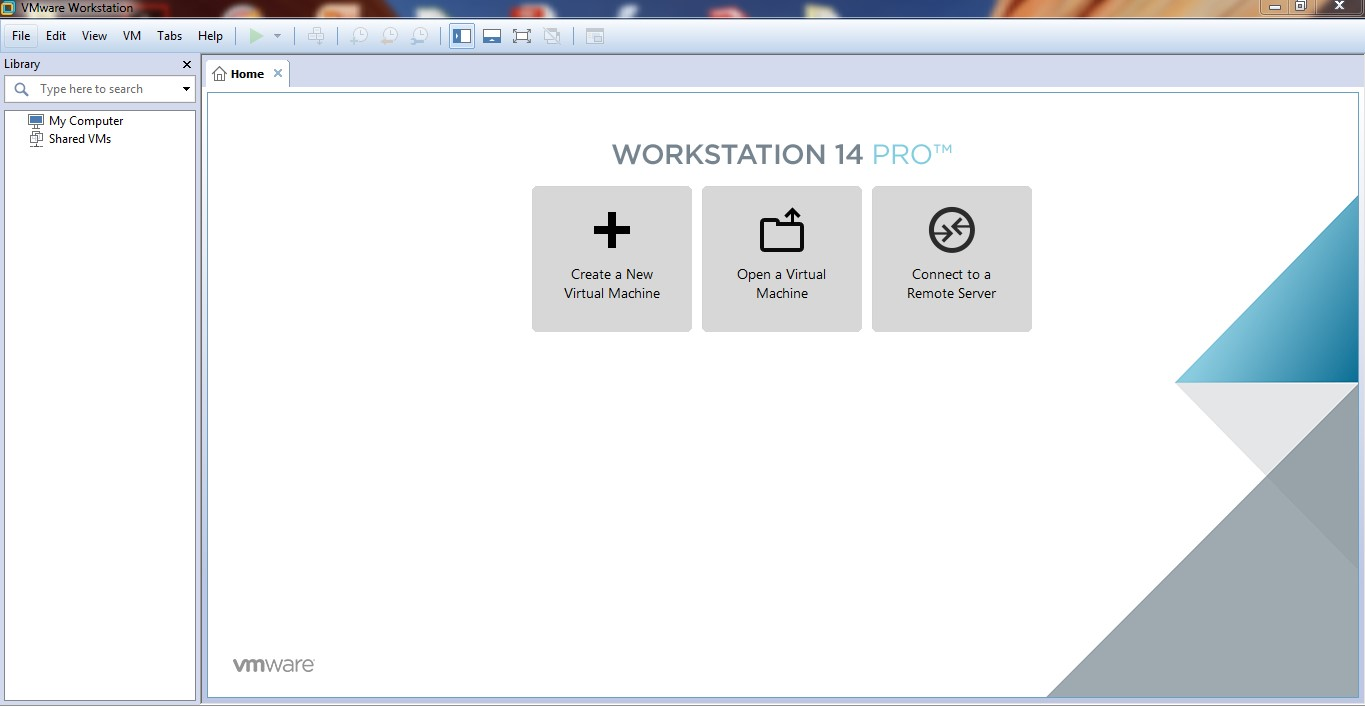
\includegraphics[width=15cm]{./Imagenes/WM10} 
	\end{center}
	
	

\end{enumerate} 

\section{Parte 03 – Instalacion de Windows Server} 

\begin{enumerate}[1.]
	\item Para virtual izar nuestro Windows Server 2012 R2, haremos uso de VMWare Workstation Pro, asignando una instalación Custom

	\begin{center}
	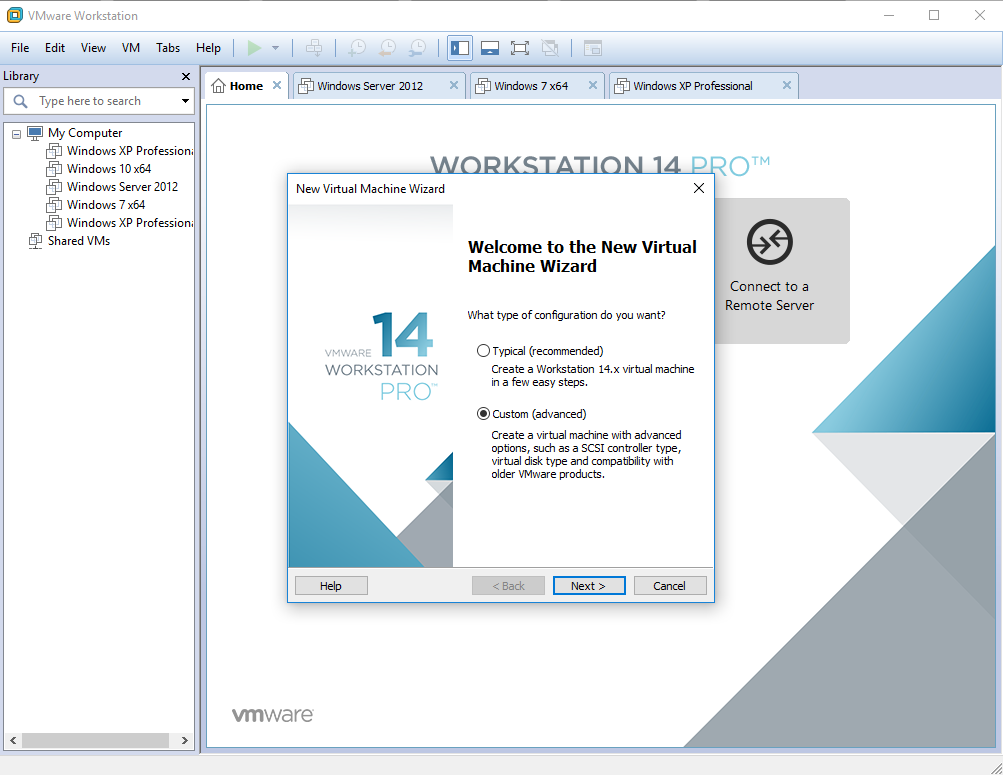
\includegraphics[width=15cm]{./Imagenes/img1server} 
	\end{center}
	
	\item Seleccionamos la tercera opción que nos permite asignar un sistema operativo después

	\begin{center}
	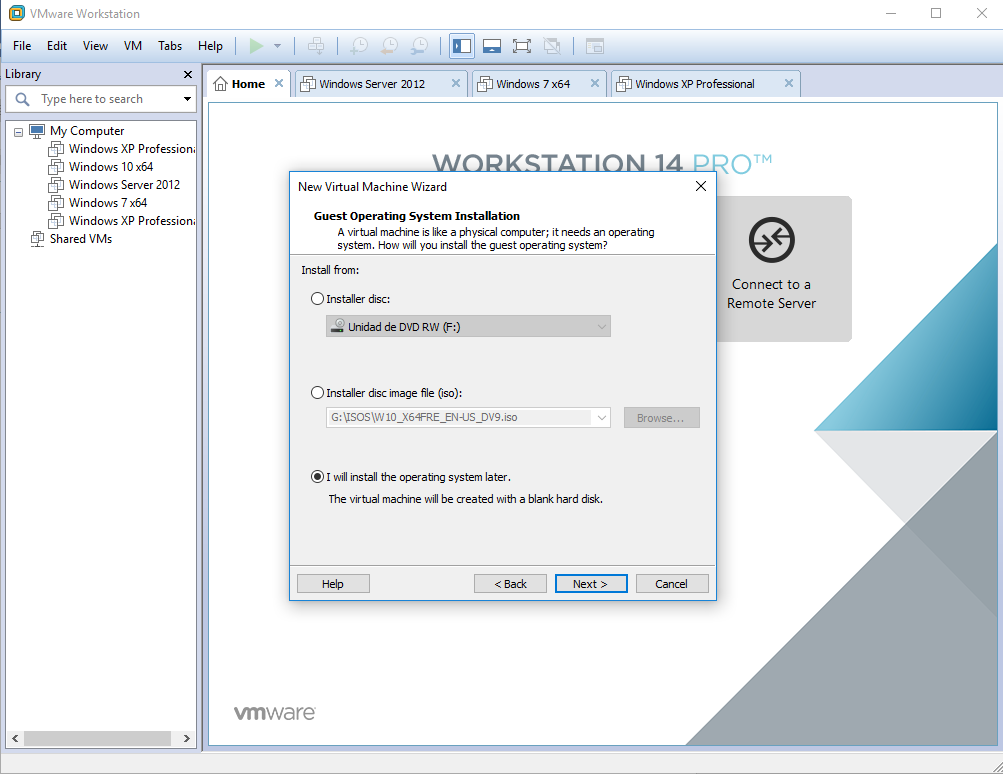
\includegraphics[width=15cm]{./Imagenes/img2server} 
	\end{center}


	\item Seleccionamos la opcion windows y buscamos en la lista Windows Server 2012

	\begin{center}
	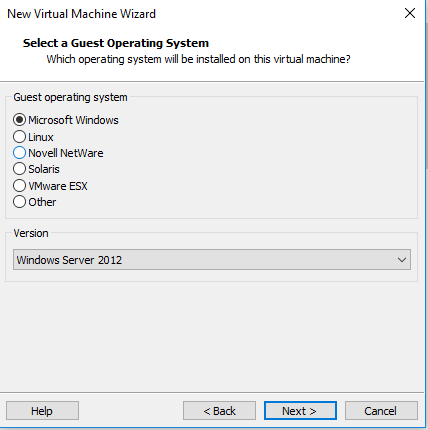
\includegraphics[width=15cm]{./Imagenes/img3server} 
	\end{center}
	
	\item Asignamos un nombre a la maquina virtual y una direccion en donde se instalara

	\begin{center}
	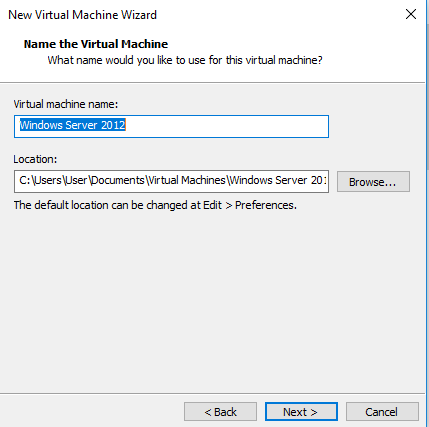
\includegraphics[width=15cm]{./Imagenes/img4server} 
	\end{center}


	\item Seleccionamos la memoria que tendra la maquina virtual

	\begin{center}
	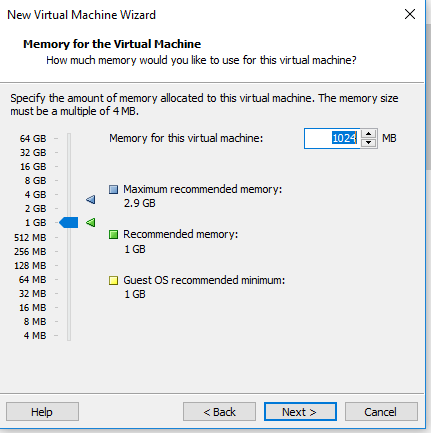
\includegraphics[width=15cm]{./Imagenes/img5server} 
	\end{center}
	
	\item Comenzamos la Instalacion

	\begin{center}
	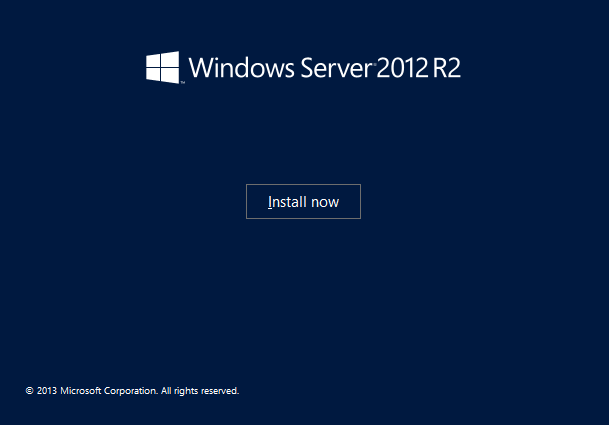
\includegraphics[width=15cm]{./Imagenes/img6server} 
	\end{center}


	\item Seleccionamos la opcion GUI

	\begin{center}
	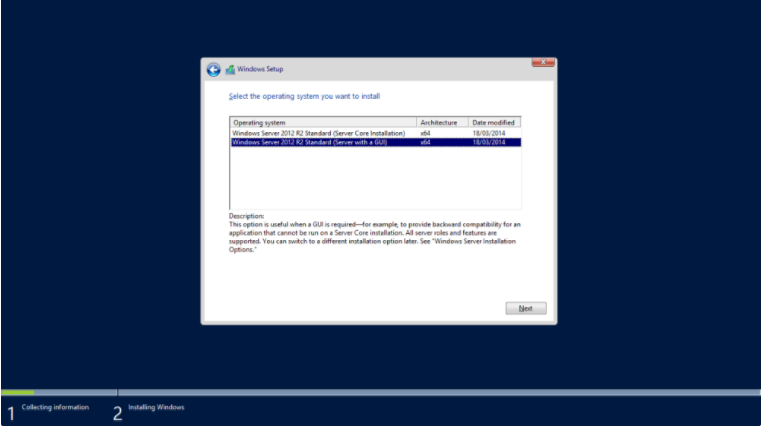
\includegraphics[width=15cm]{./Imagenes/img7server} 
	\end{center}


	\item Asignamos la contraseña Epis2018. El Administrador lo dejamos como esta

	\begin{center}
	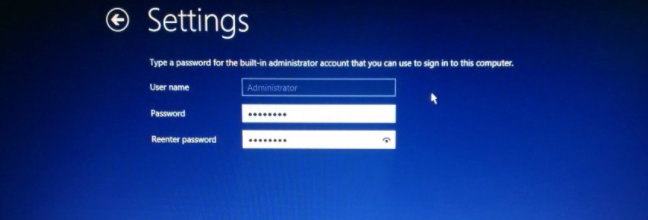
\includegraphics[width=15cm]{./Imagenes/img8server} 
	\end{center}
	
	\item siguiente paso

	\begin{center}
	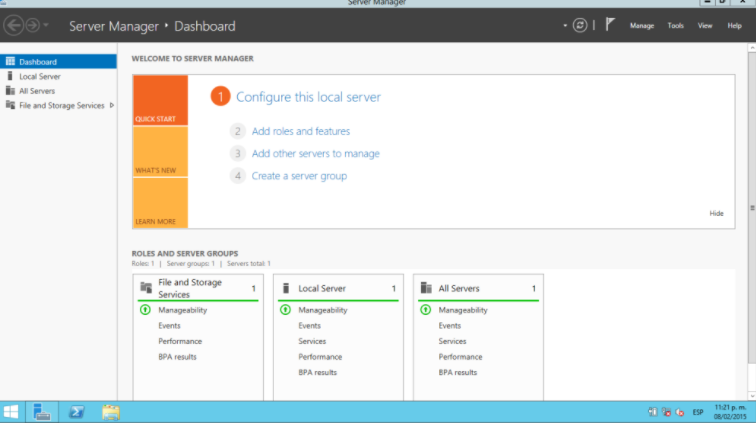
\includegraphics[width=15cm]{./Imagenes/img9server} 
	\end{center}


	\item En este laboratorio se asignará una IPv4 a cada sistema operativo para después mediante el cmd hacer ping y demostrar que están conectados.
	\subitem a)	Windows Server 2012 R2

	\begin{center}
	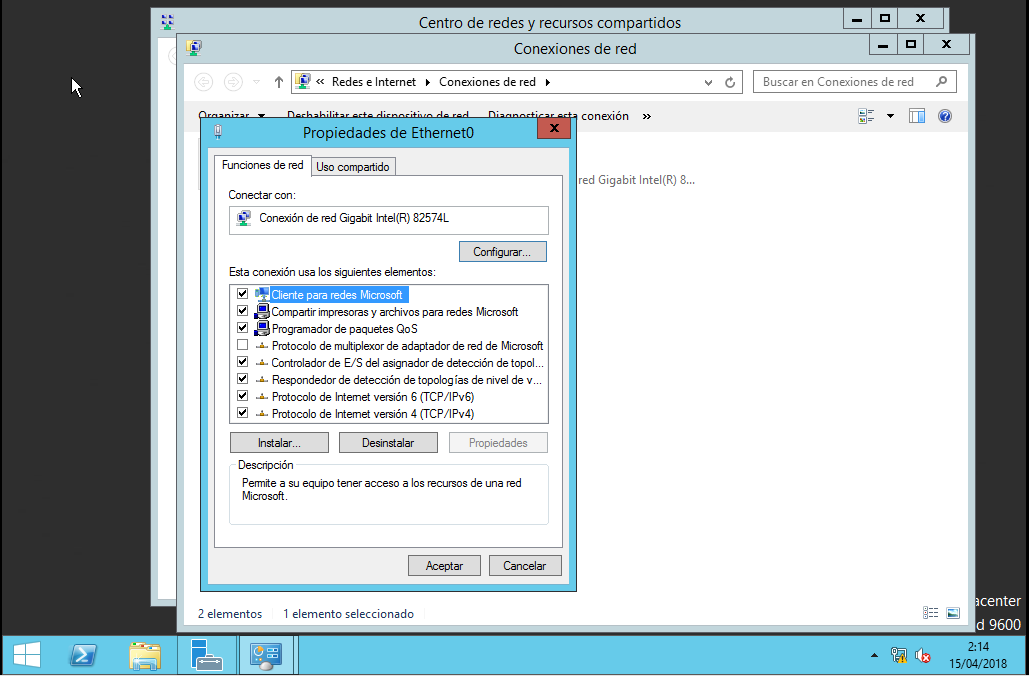
\includegraphics[width=15cm]{./Imagenes/img10server} 
	\end{center}
	
	\item Le asignamos la dirección IP que corresponde a cada estudiante determinado por el docente.

	\begin{center}
	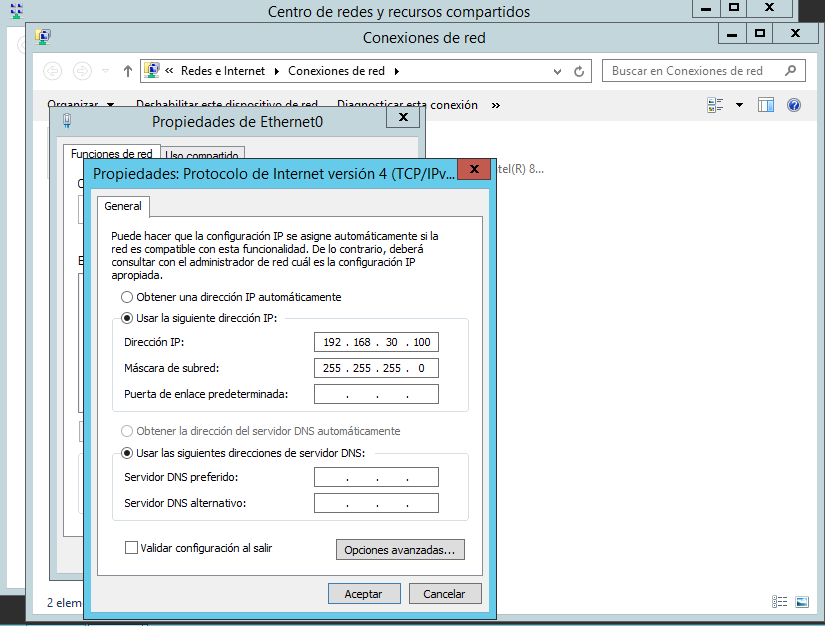
\includegraphics[width=15cm]{./Imagenes/img11server} 
	\end{center}


								

	

\end{enumerate} 

\section{Parte 04 – Instalacion de Oracle Data 12C} 

\begin{enumerate}[1.]
	\item Como primer paso para la instalaci\'on del Windows Server 2012 descargamos los iso y el archivo de instalaci\'on\\
	\begin{center}
	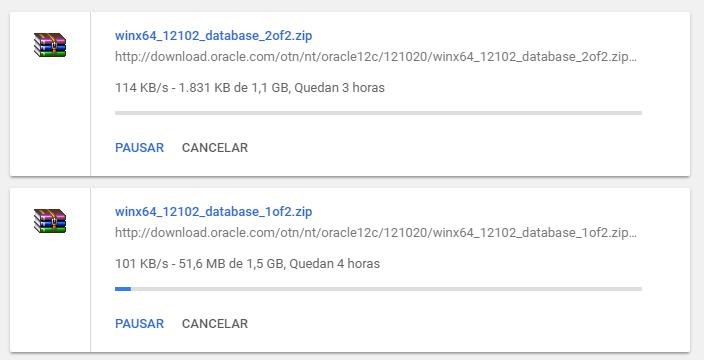
\includegraphics[width=15cm]{./Imagenes/img1} 
	\end{center}

	\item Luego ingresamos al panel de control de administrador de Windows Server\\
	\begin{center}
	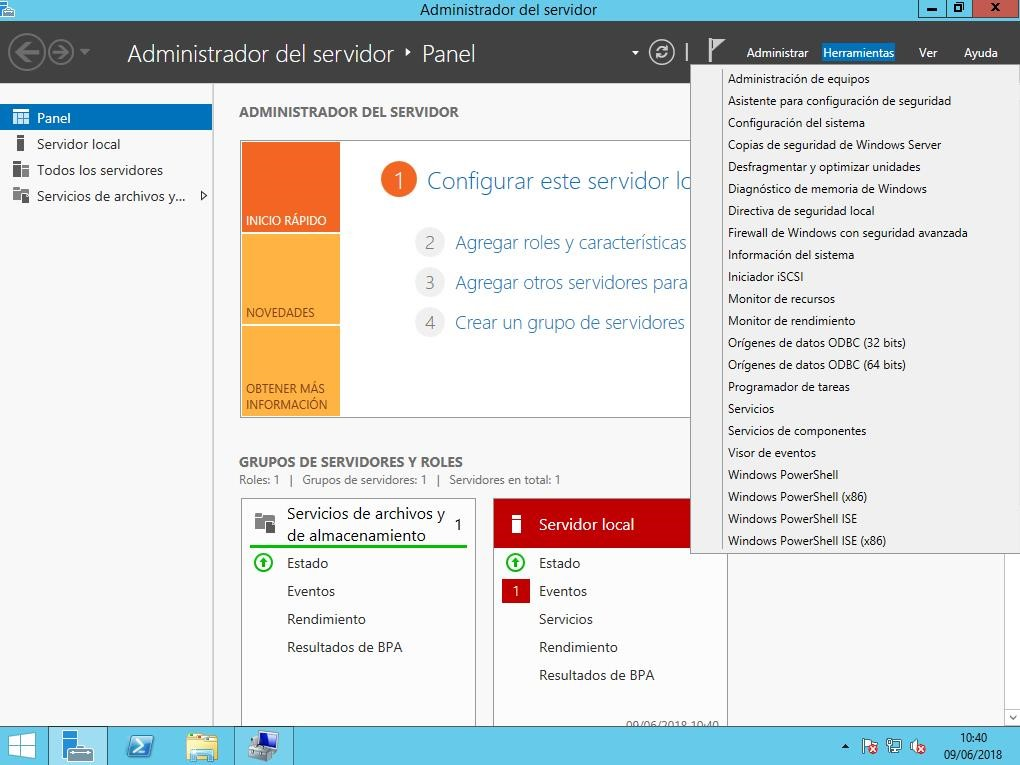
\includegraphics[width=15cm]{./Imagenes/img2} 
	\end{center}


	\item Ingresamos a la Opci\'on Administraci\'on de equipos y presionamos el bot\'on de Deshabilitada\\
	\begin{center}
	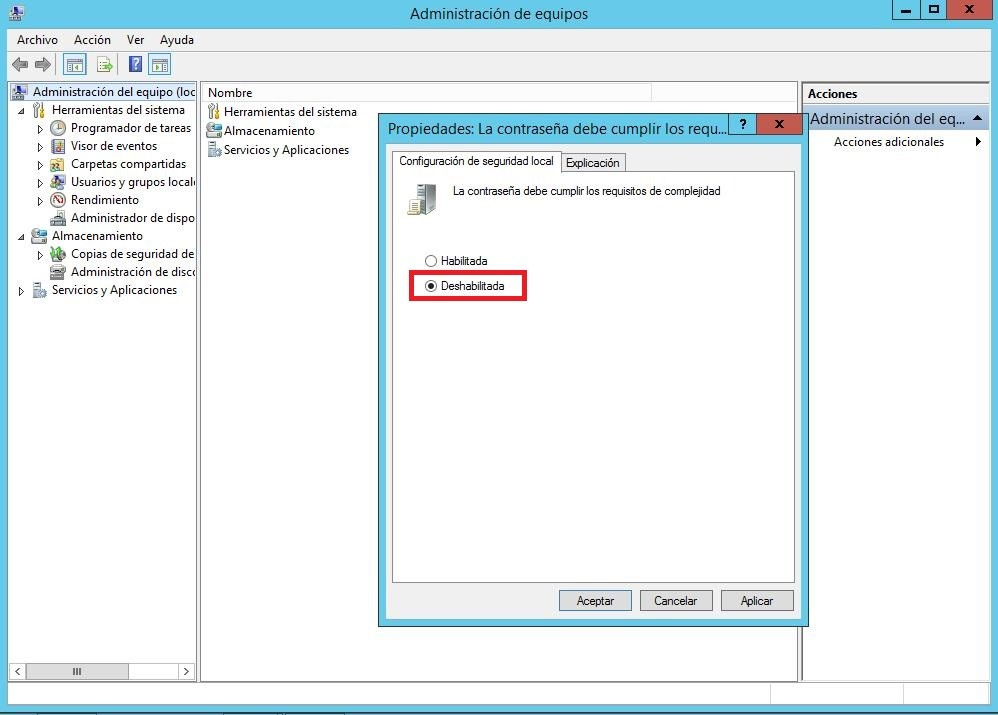
\includegraphics[width=15cm]{./Imagenes/img3} 
	\end{center}

	\item Regresamos al administrador de servicio y presionamos la opci\'on de herramientas\\
	\begin{center}
	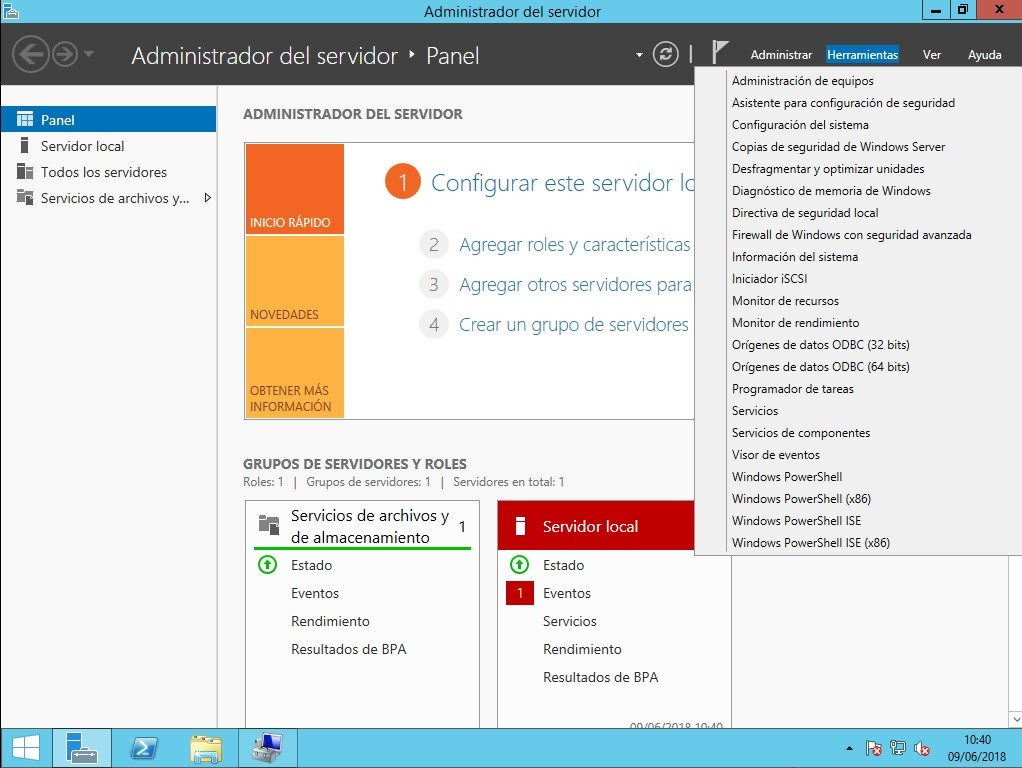
\includegraphics[width=15cm]{./Imagenes/img4} 
	\end{center}

	\item Ingresamos nuevamente Administraci\'on de equipos y nos vamos a la opci\'on de usuarios y grupos locales\\
	\begin{center}
	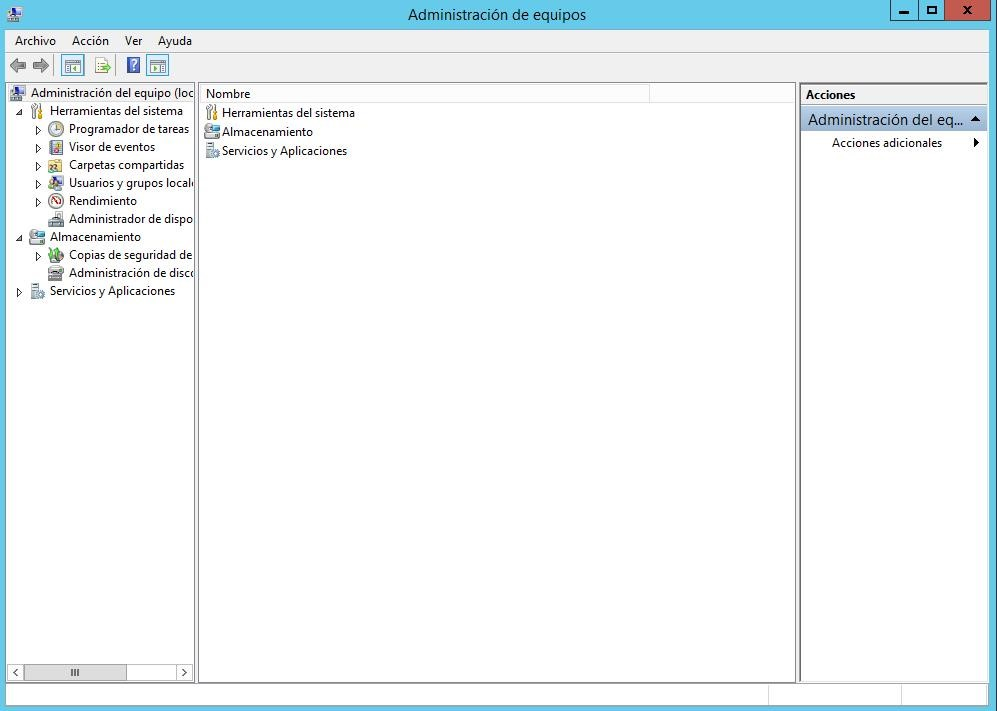
\includegraphics[width=15cm]{./Imagenes/img5} 
	\end{center}

	\item Ingresamos a la carpeta de Usuarios y nos vamos a la opci\'on de equipos ORACLE\\
	\begin{center}
	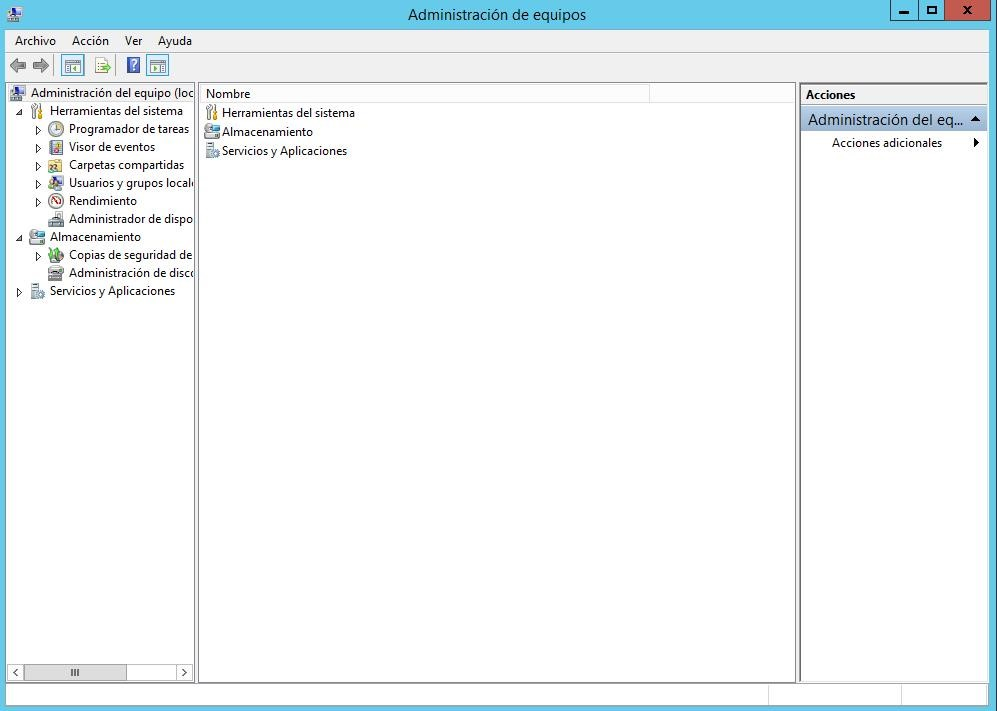
\includegraphics[width=15cm]{./Imagenes/img6} 
	\end{center}

	\item Una vez realizado eso reiniciamos el servidor y al usuario ORACLE \\
	\begin{center}
	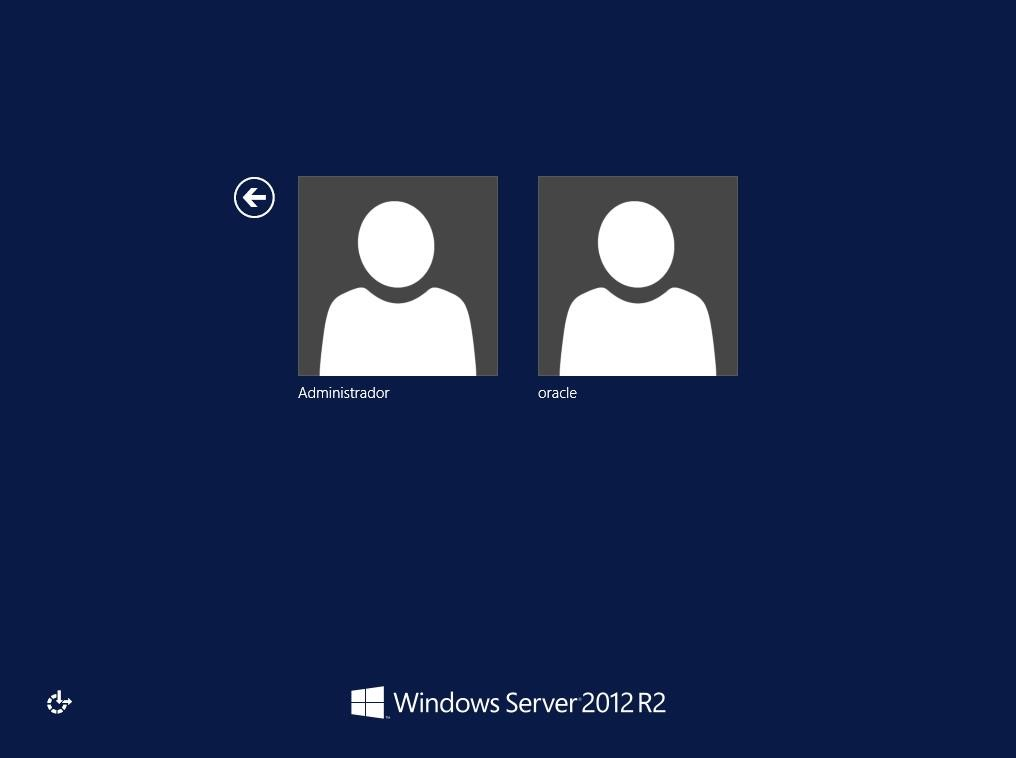
\includegraphics[width=15cm]{./Imagenes/img7} 
	\end{center}

	\item Luego colocamos la clave de administrador UPT2018\\
	\begin{center}
	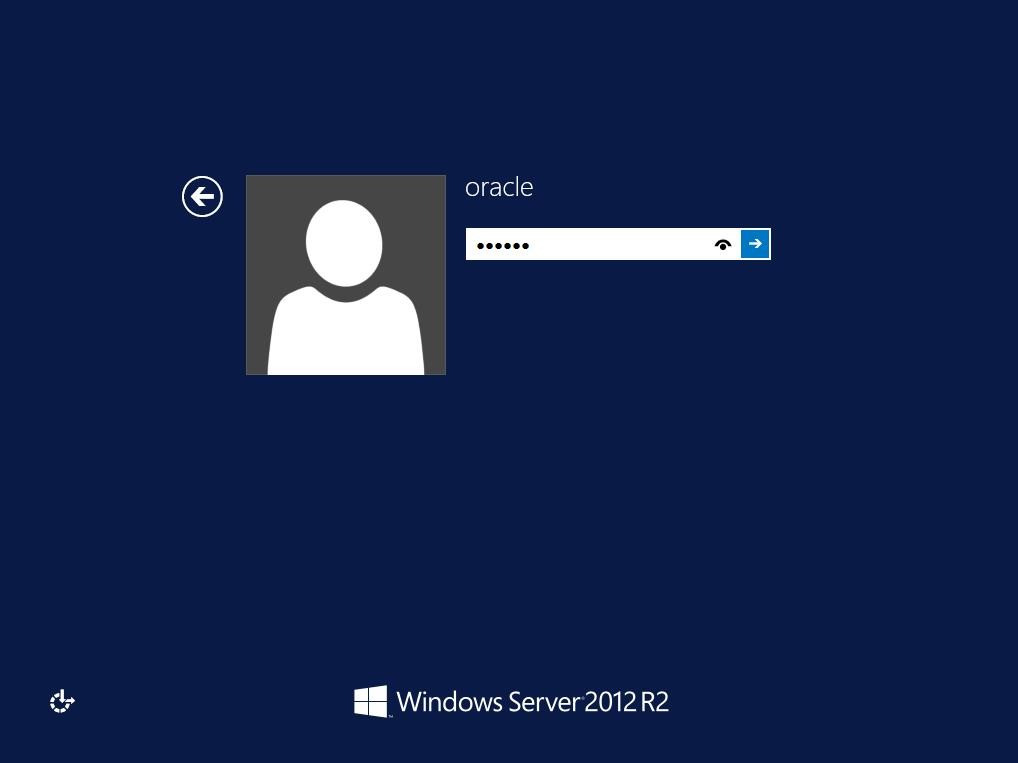
\includegraphics[width=15cm]{./Imagenes/img8} 
	\end{center}

	\item Empezaremos la instalaci\'on de la base de datos ORACLE ingresando a setup\\
	\begin{center}
	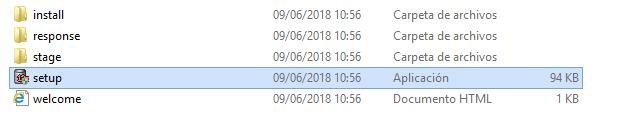
\includegraphics[width=15cm]{./Imagenes/img9} 
	\end{center}

	\item Instalamos en modo de administrador, colocando la clave de usuario\\
	\begin{center}
	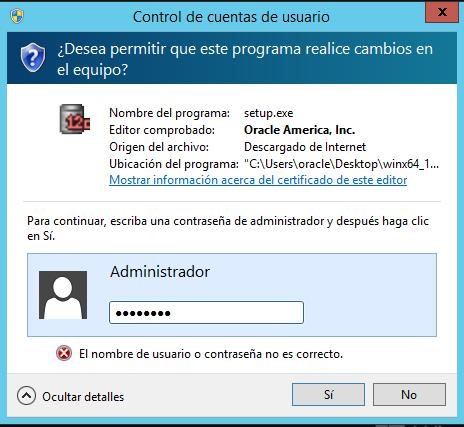
\includegraphics[width=15cm]{./Imagenes/img10} 
	\end{center}

	\item Procede autom\'aticamente la instalaci\'on del ORACLE\\
	\begin{center}
	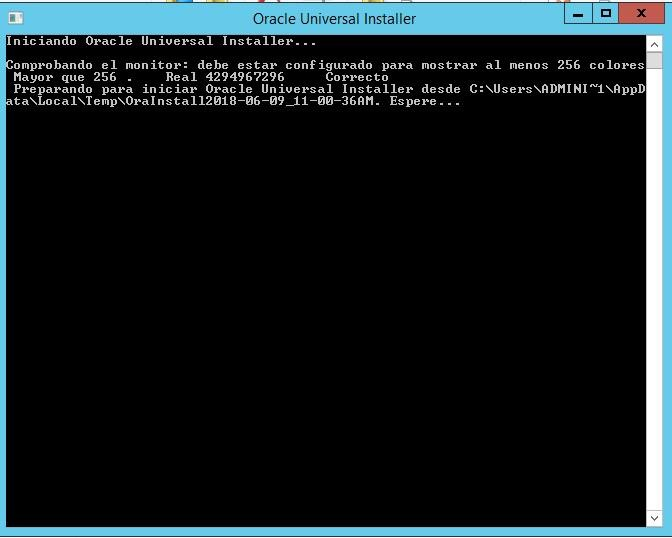
\includegraphics[width=15cm]{./Imagenes/img11} 
	\end{center}

	\item Nos aparece la pantalla de configuraci\'on \\
	\begin{center}
	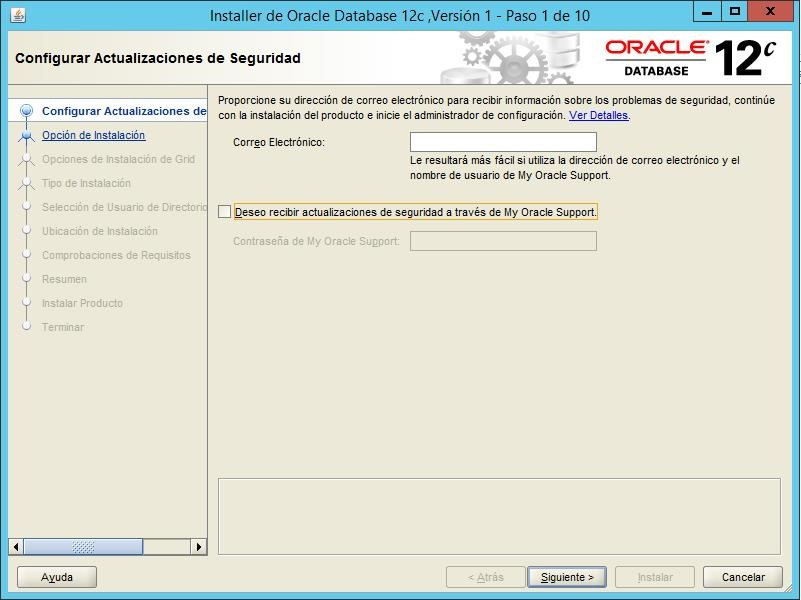
\includegraphics[width=15cm]{./Imagenes/img12} 
	\end{center}

	\item Nos saldr\'a un aviso ingresar su correo electr\'onico, colocaremos si.\\
	\begin{center}
	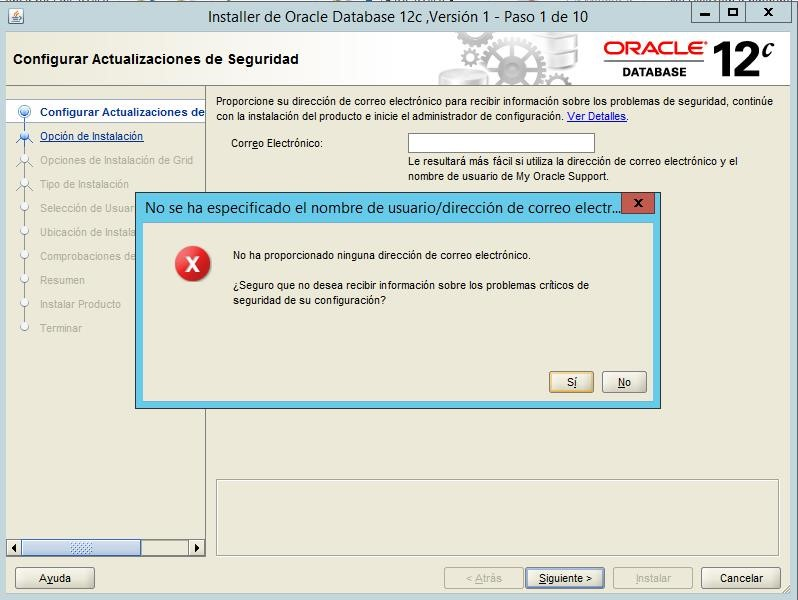
\includegraphics[width=15cm]{./Imagenes/img13} 
	\end{center}

	\item Elegimos la opci\'on de Crear y configurar Base de Datos\\
	\begin{center}
	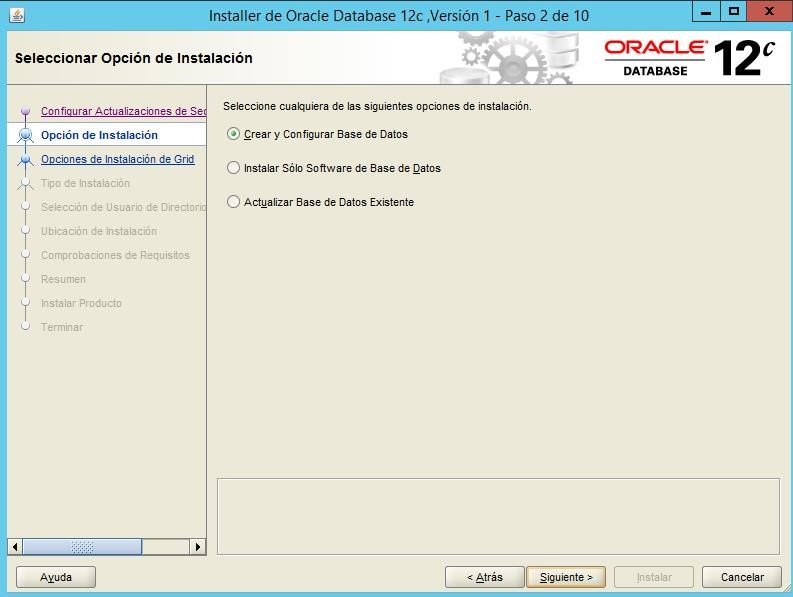
\includegraphics[width=15cm]{./Imagenes/img14} 
	\end{center}

	\item Nos aparecer\'a 2 opciones, que clase de sistema queremos instalar escogemos la opci\'on Clase escritorio\\
	\begin{center}
	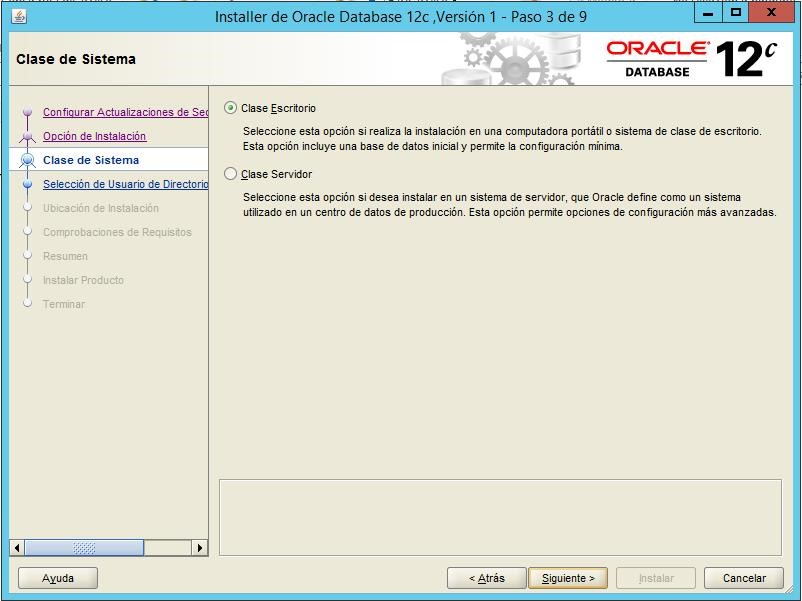
\includegraphics[width=15cm]{./Imagenes/img15} 
	\end{center}

	\item Luego ingresamos con nuestro usuario y contraseña, seleccionamos siguiente\\
	\begin{center}
	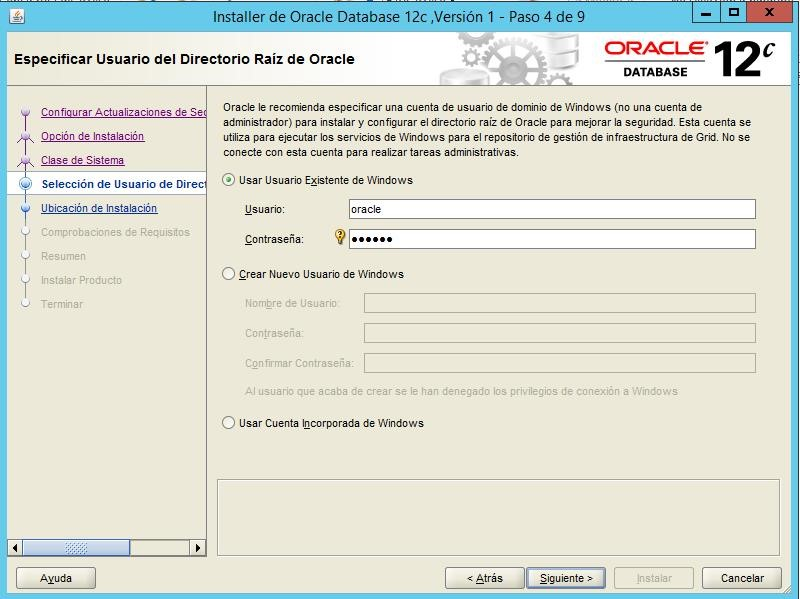
\includegraphics[width=15cm]{./Imagenes/img16} 
	\end{center}

	\item Realizamos las opciones de configuraci\'on, llenando los datos espec\'ificos\\
	\begin{center}
	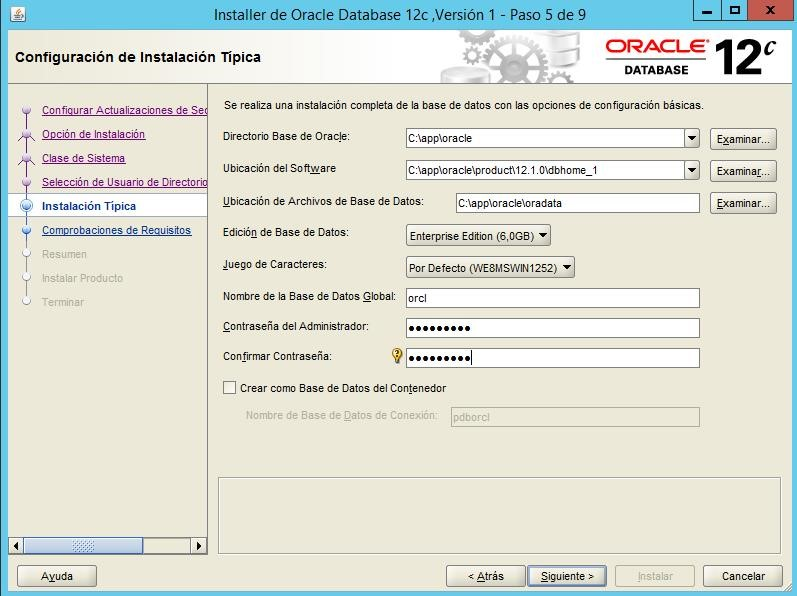
\includegraphics[width=15cm]{./Imagenes/img17} 
	\end{center}

	\item Verificaci\'on de datos y comprobaciones\\
	\begin{center}
	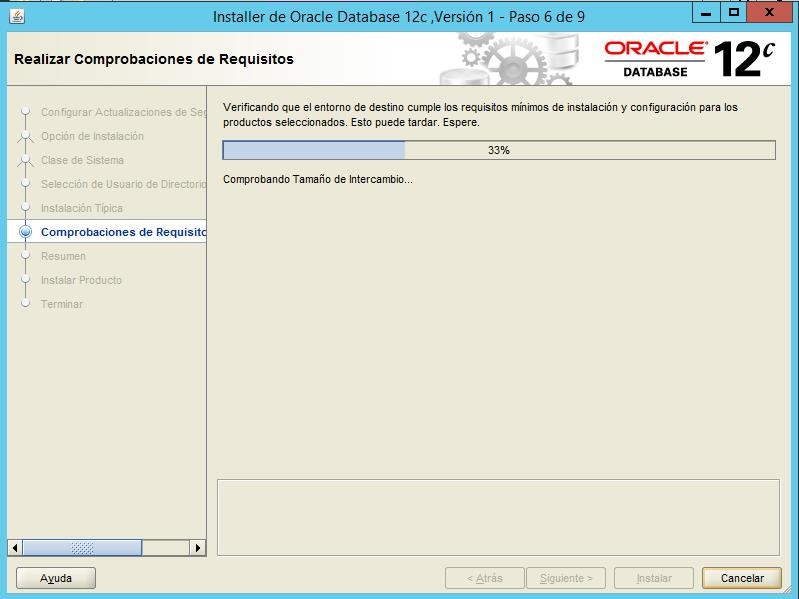
\includegraphics[width=15cm]{./Imagenes/img18} 
	\end{center}

	\item Luego nos muestra una pantalla con el Resumen de instalaci\'on\\
	\begin{center}
	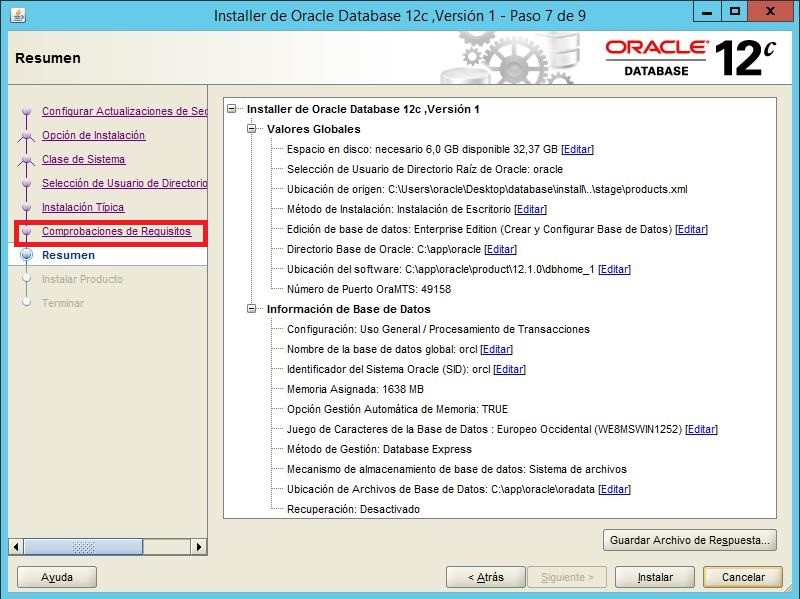
\includegraphics[width=15cm]{./Imagenes/img19} 
	\end{center}

	\item Seguidamente muestra una pantalla de comprobaci\'on nuestros requisitos y colocamos siguientes\\
	\begin{center}
	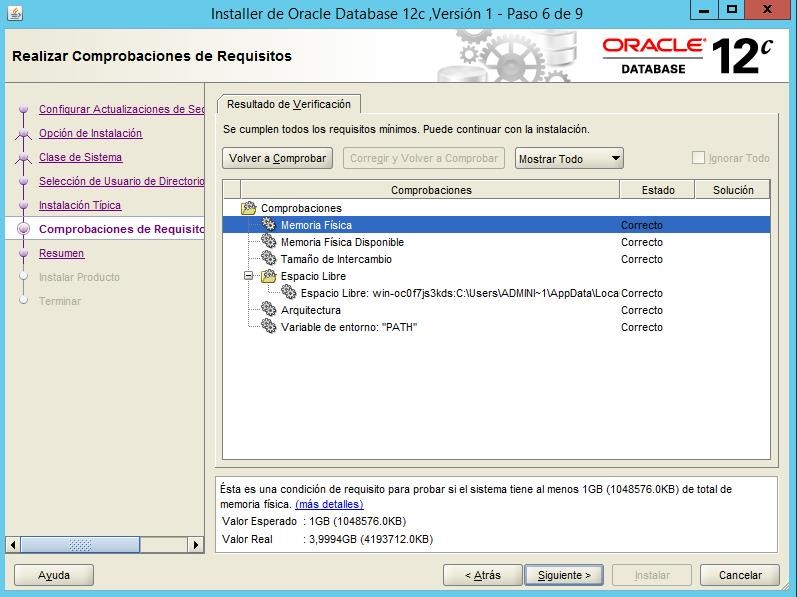
\includegraphics[width=15cm]{./Imagenes/img20} 
	\end{center}

	\item Ingresamos la opci\'on de Instalar\\
	\begin{center}
	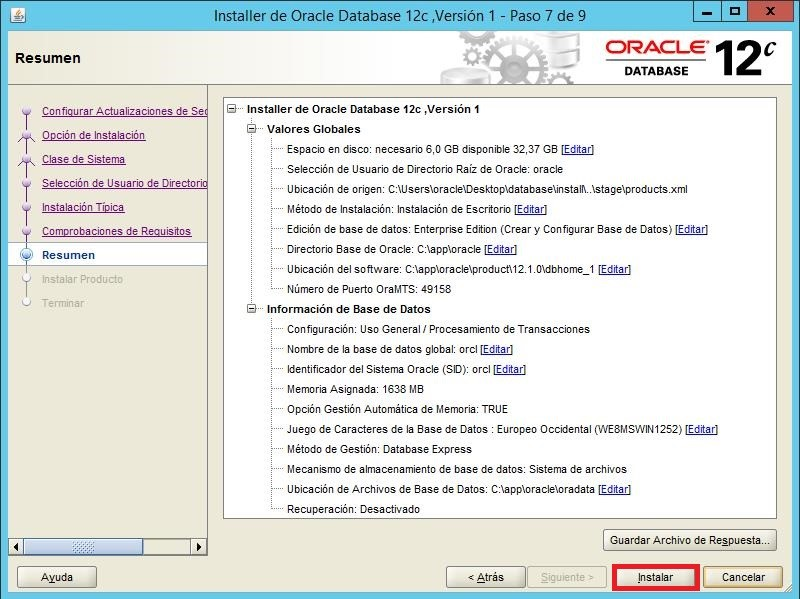
\includegraphics[width=15cm]{./Imagenes/img21} 
	\end{center}

	\item Luego esperemos la instalaci\'on de nuestro programa\\
	\begin{center}
	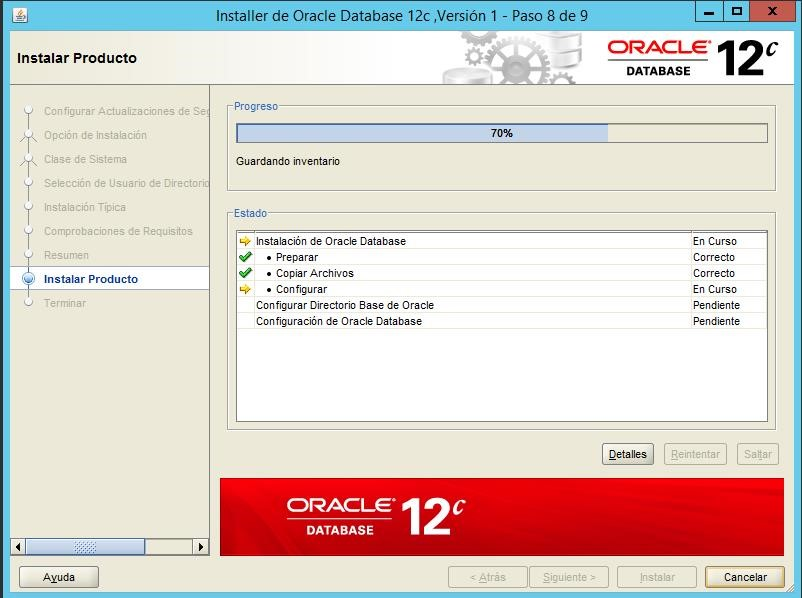
\includegraphics[width=15cm]{./Imagenes/img22} 
	\end{center}

	\item Una vez terminado colocaremos Aceptar\\
	\begin{center}
	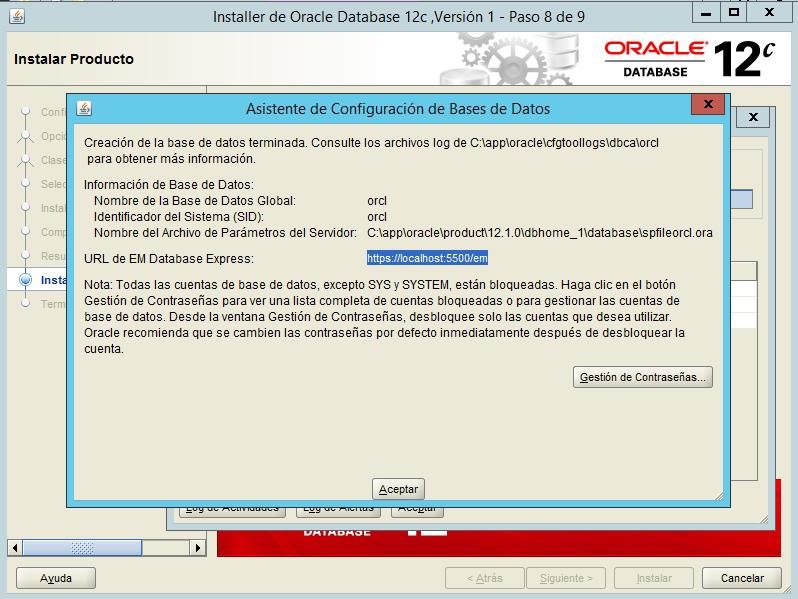
\includegraphics[width=15cm]{./Imagenes/img23} 
	\end{center}

	\item Buscamos el programa SQL DEVELOPER, seguidamente ingresamos a nuestro programa\\
	\begin{center}
	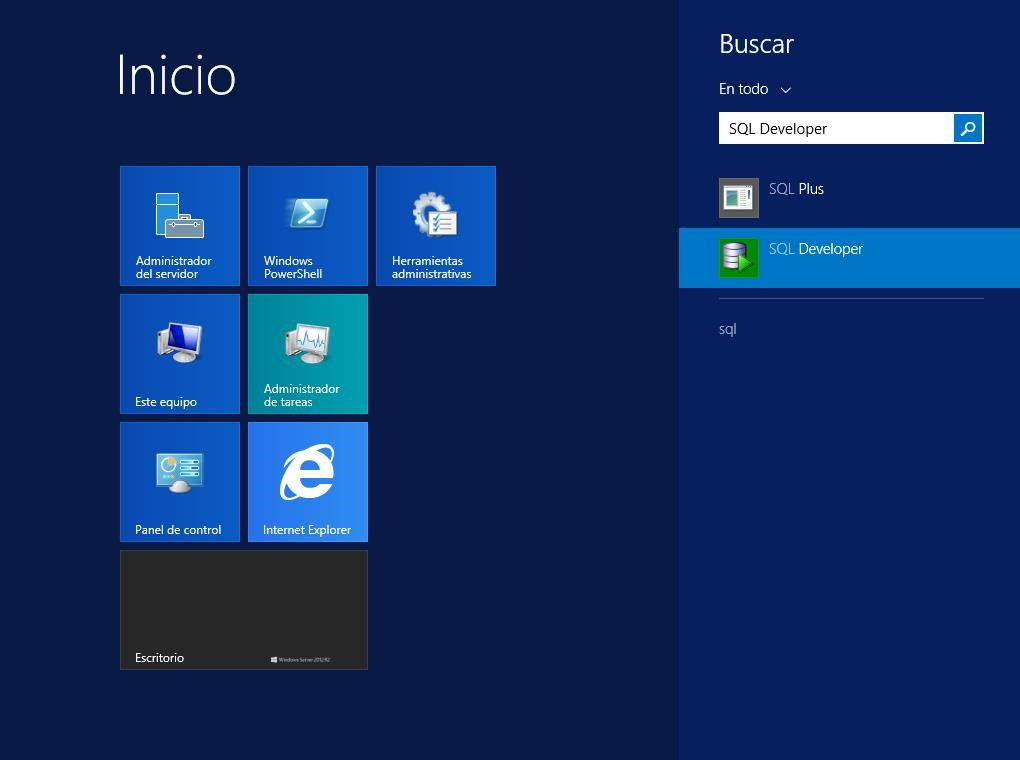
\includegraphics[width=15cm]{./Imagenes/img24} 
	\end{center}

	\item Nos saldr\'a un cuadro donde nos pedir\'a que ingresemos nuestra clave de administrador\\
	\begin{center}
	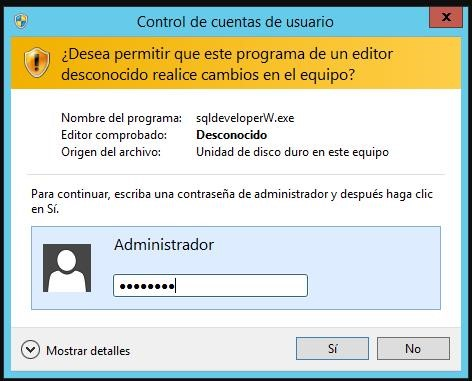
\includegraphics[width=15cm]{./Imagenes/img25} 
	\end{center}

	\item Ingresamos a la opci\'on de Nueva conexi\'on\\
	\begin{center}
	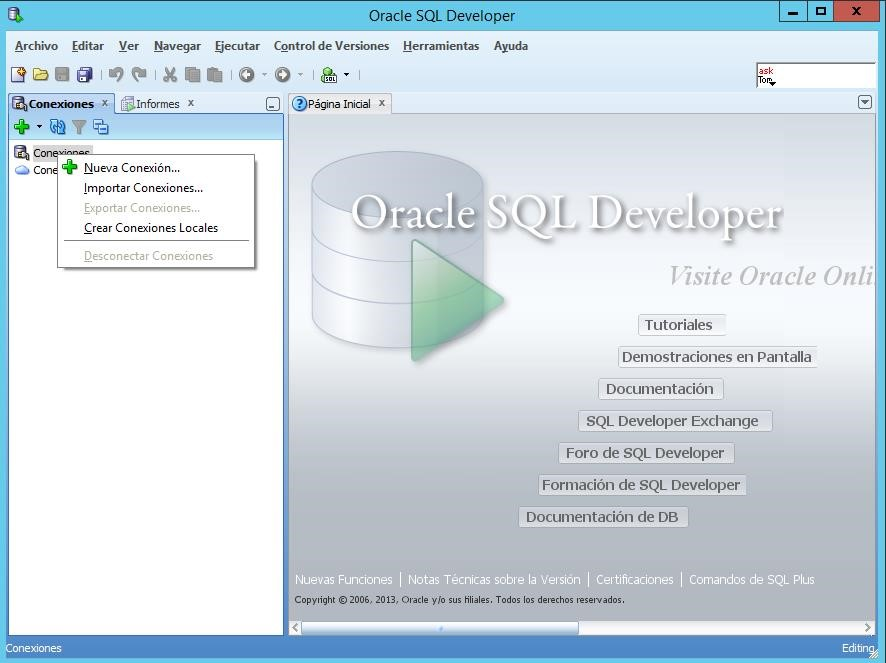
\includegraphics[width=15cm]{./Imagenes/img26} 
	\end{center}

	\item Crearemos nuestra nueva conexi\'on de datos, ingresando todos los datos correspondientes, una vez echo eso colocaremos probar\\
	\begin{center}
	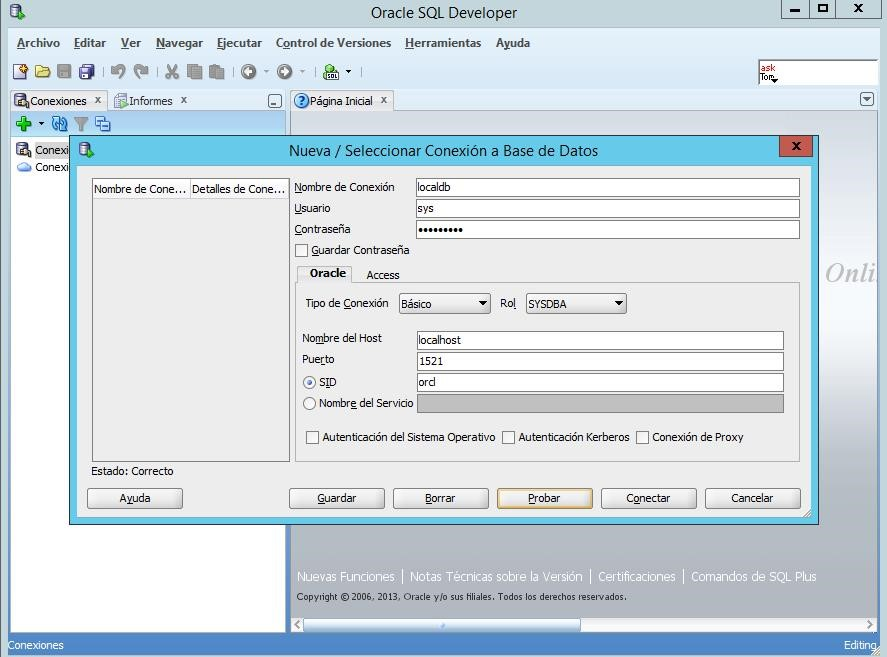
\includegraphics[width=15cm]{./Imagenes/img27} 
	\end{center}

	\item Luego observamos nuestra base de datos creada y lista para su funcionamiento\\
	\begin{center}
	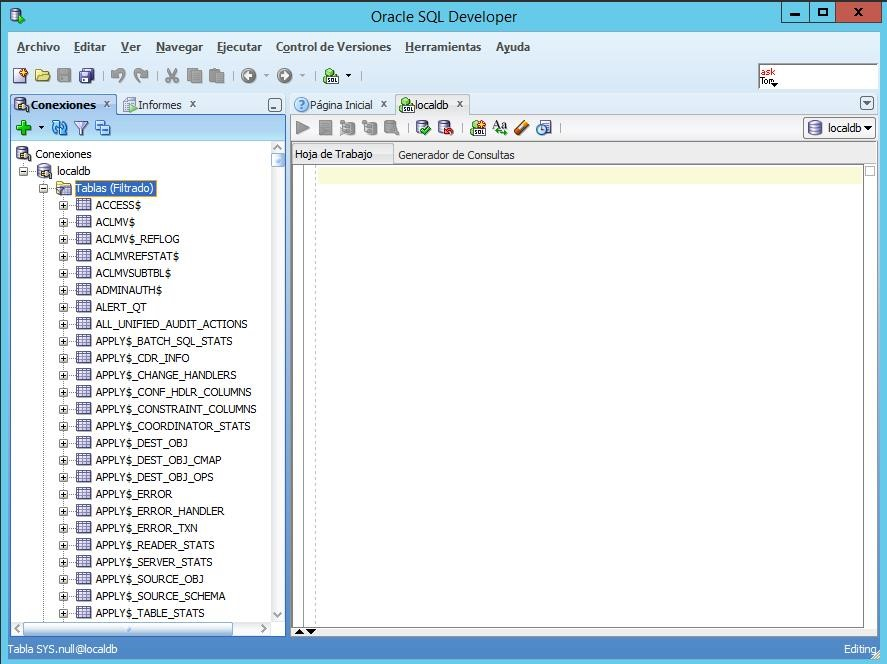
\includegraphics[width=15cm]{./Imagenes/img28} 
	\end{center}


\end{enumerate} 

\include{Secciones/Actividad05}



\end{document}
